\documentclass[a4j,12pt,onecolumn,oneside,titlepage,openany,final]{jreport}
\setlength{\topmargin}{0cm}
\setlength{\oddsidemargin}{0cm}
\setlength{\textwidth}{16cm}

\usepackage[dvipdfmx]{graphicx}
\usepackage{url}
\usepackage{comment} %コメントアウト
\usepackage{here} %図の強制表示
\renewcommand{\bibname}{参考文献}
\setcounter{secnumdepth}{4}
\usepackage{listings}
\usepackage[dvipdfmx]{xcolor}
\definecolor{background}{HTML}{EEEEEE}
\lstdefinelanguage{http}{
basicstyle=\normalfont\ttfamily,
numbers=left,
numberstyle=\scriptsize,
stepnumber=1,
numbersep=8pt,
showstringspaces=false,
breaklines=true,
frame=lines,
backgroundcolor=\color{background},
}

\title{
% 1行に入るなら行を分ける必要はないよ
 \Huge{スマートフォン用K'sLifeアプリ}\\
 \Huge{「スマト君」の開発}
 \vspace{5.5cm}\\
}
\author{\LARGE{16JK053}\vspace{0.5cm}\\
\LARGE{NGUYEN THANH LONG}\vspace{2cm}\\
\LARGE{九州産業大学 情報科学部}\vspace{0.5cm}\\
\LARGE{情報科学科}\vspace{1cm}\\
\date{\LARGE{令和2年1月}}
}
\pagestyle{plain}
\begin{document}


\maketitle
\tableofcontents
\listoffigures
\listoftables



%-----------------------------------------------------------------------------------------------------------------

\chapter{序論}\label{joron}

本章では研究背景、研究目的、論文構成について述べる。
\section{研究背景}\label{haikei}
九州産業大学では、学生教育支援・事務情報システム K'sLife\cite{kslife} が運用されている。
K'sLife は、履修登録や成績確認、連絡通知、週間スケジュールなど様々な機能がある。
また、K'sLifeにはパソコン版のページとスマートフォン版のページがある。
しかし、スマートフォン版のページは利便性が低くあまり使われていない。



\section{研究目的}\label{mokuteki}
本研究の目的は、K'sLife にアクセスするための、使い勝手の良いスマートフォン用アプリケーションを開発することである。
\section{論文構成}\label{kousei}
本論文の構成は全7章からなり、構成は以下の通りである。
\ref{mondai}章では、スマートフォンでのK'sLifeの利用について述べる。
\ref{sumatokun}章では、スマト君について述べる。
\ref{api}章では、スマト君 API Serverについて述べる。
\ref{smartphone}章では、スマートフォンアプリケーションについて述べる。
\ref{keturon}章では、本研究のまとめと今後の課題について述べる。

%-----------------------------------------------------------------------------------------------------------------

\chapter{スマートフォンでのK'sLifeの利用}\label{mondai}
 K'sLifeとは九州産業大学の学生教育支援・事務情報システムである。
本章では、K's Lifeをスマートフォンで使用するときの問題点について述べる。

\section{問題点}\label{mondaiten}
K'sLife をスマートフォンで使用するとき、以下の問題点がある。
\begin{itemize}
\item 毎回ログインしなければならない
\item スマートフォン版の操作はステップが多い
\item パソコン版はスマートフォンで操作しにくい
\item トップページに未読通知しか載ってない
\item 既読の通知を再度見たいときの操作はステップが多い
\item 新しい連絡が来ても、通知される機能がない
 \end{itemize}

\section{解決策}\label{kaisaku}
 2.1 で述べた問題点を解決するために、本研究では専用のスマートフォン用アプリケーションを開発する。
 本アプリケーションを「スマト君」と名付ける。

%-----------------------------------------------------------------------------------------------------------------

\chapter{スマト君}\label{sumatokun}
本章では、スマト君について述べる。
\section{スマト君の機能}\label{kizon_gaiyou}
スマト君の機能は以下の通りである。
\begin{itemize}
\item 自動ログイン機能
\\K‘sLife に自動ログイン
\item 時間割参照機能
\\時間割を表示
\item 連絡通知参照機能
\\未読通知と既読通知を区別して表示
\item 出欠情報参照機能
\\出欠状況を表示
\item スケジュール参照機能
\\スケジュールを表示
\item 通知機能
\\新しい連絡を通知

\end{itemize}

\section{スマト君の構成}\label{kizon_database}
スマト君は K'sLife のデータを表示するスマートフォン用アプリケーションである。
すなわち、K'sLife のデータを取得する必要がある。
しかし K'sLife は Web API を提供していない。
そこで本研究では、独自に K'sLife の Web API を提供するためのサーバを開発した。

これら全体を「スマト君システム」と呼ぶ。スマト君の全体の構成を図\ref{kousei} に示す。
スマト君は以下の3つの部分から構成される。
\begin{itemize}
\item K'sLife
\item Web API server
\item スマートフォン用アプリケーション
\end{itemize}

このうち、Web API server を「スマト君 API Server」と呼ぶ。
また、スマートフォン用アプリケーションを「スマト君アプリケーション」と呼ぶ。
\begin{figure}[htbp]
  \centering %中央寄せ
  \fbox{
    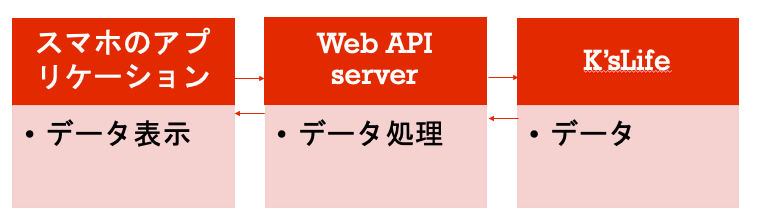
\includegraphics[clip,width = 13cm]{kousei.png} %読み込む画像
  }
\caption{スマト君システム全体の構成}\label{kousei}
\end{figure}

%-----------------------------------------------------------------------------------------------------------------

\chapter{スマト君 API Server}\label{api}
本章ではスマト君 API Serverについて述べる

\section{概要}\label{rihabiri_jisso}
スマト君API Serverは、スマト君アプリケーションから HTTP でリクエストを受け、K'sLife にアクセスし、その結果を解析し JSON データとしてスマト君アプリに返す。

\section{スマト君 API Serverの設計と性能の比較}
12個エンドポイントで以下の3種類のAPIを設計した。
\subsection{各データを別々に取得するAPI}\label{api}
データを別々に取得するAPIである。
表\ref{uri}に示す9個エンドポイントから構成されている。
表中の実行時間は、各エンドポイントの実行時間を5回計測した平均である。
\begin{table}[htbp]
\caption{各データを別々に取得するAPI}
\begin{tabular}{|l|l|l|r|}
\hline
   & 機能         & エンドポイント    & \multicolumn{1}{l|}{実行時間} \\ \hline
1  & 名前,学籍番号を取得 & POST /name & 2712.550                   \\ \hline
2  & 時間割を取得                        & POST /timetable            & 4586.776    \\ \hline
3  & スケジュールを取得                     & POST /schedule             & 2803.907    \\ \hline
4  & 出欠を取得                         & POST /attendance           & 3804.002    \\ \hline
5  & 出欠詳細を取得                       & POST /attendance\_detail   & 3824.957    \\ \hline
6  & 学内連絡を取得                       & POST /campus\_noti         & 4766.843    \\ \hline
7  & 学内連絡詳細を取得                     & POST /campus\_noti\_detail & 3834.630     \\ \hline
8  & 授業連絡を取得                       & POST /class\_noti          & 5495.575    \\ \hline
9  & 授業連絡詳細を取得                     & POST /class\_noti\_detail  & 5922.901    \\ \hline
\end{tabular}
\label{uri}
\end{table}
\subsection{データを一緒に取得するAPI}\label{api1}
データを一緒に一回で全部取得するAPIである。
表\ref{uri1}に示す6個エンドポイントから構成されている。
表内の実行時間は、表\ref{uri} と同じである。
\begin{table}[htbp]
\caption{データを一緒に取得するAPI}
\begin{tabular}{|l|l|l|r|}
\hline
   & 機能         & エンドポイント    & \multicolumn{1}{l|}{実行時間} \\ \hline
1  & 出欠詳細を取得                       & POST /attendance\_detail   & 3824.957    \\ \hline
2  & 学内連絡を取得                       & POST /campus\_noti         & 4766.843    \\ \hline
3  & 学内連絡詳細を取得                     & POST /campus\_noti\_detail & 3834.630     \\ \hline
4  & 授業連絡を取得                       & POST /class\_noti          & 5495.575    \\ \hline
5  & 授業連絡詳細を取得                     & POST /class\_noti\_detail  & 5922.901    \\ \hline
6 & 名前、連絡通知、出欠、スケジュール、時間割を取得 & POST /all                  & 9239.430     \\ \hline
\end{tabular}
\label{uri1}
\end{table}
\subsection{データを2回で取得するAPI}\label{api2}
データを2回分けて取得するAPIである。
表\ref{uri2}に示す7個エンドポイントから構成されている。
表内の実行時間は、表\ref{uri} と同じである。
\begin{table}[htbp]
\caption{データを2回で取得するAPI}
\begin{tabular}{|l|l|l|r|}
\hline
   & 機能         & エンドポイント    & \multicolumn{1}{l|}{実行時間} \\ \hline
1  & 出欠詳細を取得                       & POST /attendance\_detail   & 3824.957    \\ \hline
2  & 学内連絡を取得                       & POST /campus\_noti         & 4766.843    \\ \hline
3  & 学内連絡詳細を取得                     & POST /campus\_noti\_detail & 3834.630     \\ \hline
4  & 授業連絡を取得                       & POST /class\_noti          & 5495.575    \\ \hline
5  & 授業連絡詳細を取得                     & POST /class\_noti\_detail  & 5922.901    \\ \hline
6 & 名前、学籍番号、時間割を取得                & POST /name\_timetable      & 3512.081    \\ \hline
7 & 出欠、スケジュール、連絡通知を取得             & POST /all2                 & 7156.166\\ \hline
\end{tabular}
\label{uri2}
\end{table}
\subsection{性能の比較}


3つ設計したAPIの性能の実行時間を比較した。
\ref{api}で述べた各データを別々に取得するAPIを用いる場合、
すべての情報を取得するためには6つのAPI全てにアクセスする必要がある。
6つのAPIに順にアクセスした場合、実行時間が長いという問題がある。
これを解決するために、6つのAPIに並列にアクセスする方法がある。
しかし、この方法はサーバに過負荷を掛けることになる。
したがって、本APIは不採用とした。
\ref{api1}で述べた、データを一緒に取得するAPIは実行時間が長い。
初回ログイン時に実行する POST /all の実行時間は9秒以上かかる。
また、初回アクセス時に全てのデータを必要とするわけでもない。
したがって、不採用とした。
\ref{api2} で述べた、データを2回で取得するAPIは、上述の2つのAPIの問題を解決する。
初回アクセス時に実行する POST /all2 の実行時間は7秒程度である。
そして、K'sLifeにブラウザーの1つタブしか使わない。
したがって、このAPIを使用することにした。



\section{スマト君 API Server の API}\label{rihabiri_jisso}
今回開発したすべての API は、ログイン用の ID とパスワードを引数として与える。
K'sLife は、ログインしたまま長時間経過すると、自動でログアウトしてしまう。このため、スマト君API Server は、ログイン状態を維持するのではなく、K'sLife にアクセスする度に毎回ログインし、データを取得後ログアウトする。
この際、スマト君 API Server上で、ID やパスワードを管理するのはセキュリティ上のリスクが有る。そこで、API の引数としてこれらの情報を与える。

スマト君API Server の API は7個のエンドポイントで構成されている。
以下で、それぞれのエンドポイントについて説明する。
\subsection{名前、学籍番号、時間割を取得}
ログインするユーザの名前、学籍番号、時間割を取得するAPIである。
\begin{lstlisting}[language=http, firstnumber=1]
POST /name_timetable
\end{lstlisting}

\subsubsection{インプット}
インプットを表\ref{input}に示す。

\begin{table}[htbp]
  \caption{共通のインプット}
  \centering
\begin{tabular}{lllll}
\cline{1-3}
\multicolumn{1}{|l|}{Name} & \multicolumn{1}{l|}{Type}   & \multicolumn{1}{l|}{Description} &  &  \\ \cline{1-3}
\multicolumn{1}{|l|}{id}   & \multicolumn{1}{l|}{String} & \multicolumn{1}{l|}{ログイン用ID}     &  &  \\ \cline{1-3}
\multicolumn{1}{|l|}{pas}  & \multicolumn{1}{l|}{String} & \multicolumn{1}{l|}{ログイン用パスワード}  &  &  \\ \cline{1-3}
                           &                             &                                  &  &
\end{tabular}
\label{input}
\end{table}

\subsubsection{レスポンス}
レスポンスを表\ref{timetable}に示す。
\begin{table}[htbp]
\caption{POST /name\_timetableのレスポンス}
\centering
\begin{tabular}{|l|l|}
\hline
Key                    & Description                    \\ \hline
name                   & 学生の氏名と学籍番号 \\ \hline
name{[}student\_id{]}  & 学籍番号                           \\ \hline
name{[}name{]}         & 学生の氏名                          \\ \hline
timetable              & 時間割                            \\ \hline
timetable{[}subject{]} & 科目                             \\ \hline
timetable{[}teacher{]} & 先生                             \\ \hline
timetable{[}room{]}    & 教室                             \\ \hline
\end{tabular}
\label{timetable}
\end{table}
\subsection{出欠、スケジュール、連絡通知を取得}
ログインするユーザの出欠、スケジュール、連絡通知を取得するAPIである。
\begin{lstlisting}[language=http, firstnumber=1]
 POST /all2
\end{lstlisting}
 \subsubsection{インプット}

 インプットを表\ref{input}に示す。
 \subsubsection{レスポンス}
 レスポンスを表\ref{all2}に示す。

 \begin{table}[htbp]
 \caption{POST /all2のレスポンス}
 \centering
 \begin{tabular}{|l|l|}
 \hline
 Key                    & Description                    \\ \hline
 attendance                   & 出欠情報 \\ \hline
 attendance{[}no{]}  & 科目の番号                           \\ \hline
 attendance{[}subject{]}         & 科目                          \\ \hline
 attendance{[}time{]}              & 時間                            \\ \hline
 schedule & スケジュール                             \\ \hline
 schedule{[}date{]} & 時間                          \\ \hline
 schedule{[}event{]} & イベント                             \\ \hline
 camp & 学内連絡                             \\ \hline
 camp{[}no{]} & 情報の番号                             \\ \hline
 camp{[}unread{]} & 未読か既読                             \\ \hline
 camp{[}title{]} & タイトル                             \\ \hline
  camp{[}time{]} & 時間                             \\ \hline
  class & 授業連絡                             \\ \hline
  class{[}no{]} & 情報番号                             \\ \hline
  class{[}unread{]} & 未読か既読                               \\ \hline
  class{[}title{]} & タイトル                                 \\ \hline
   class{[}time{]} & 時間                             \\ \hline

 \end{tabular}
 \label{all2}
 \end{table}
\subsection{出欠詳細を取得}

\begin{lstlisting}[language=http, firstnumber=1]
POST /attendance_detai
\end{lstlisting}
\subsubsection{インプット}

インプットを表\ref{input2}に示す。

\begin{table}[htbp]
  \caption{指定情報がある共通のインプット}
\centering
\begin{tabular}{|l|l|l|ll}
\cline{1-3}
Name & Type   & Description &  &  \\ \cline{1-3}
id   & String & ログイン用ID     &  &  \\ \cline{1-3}
pas  & String & ログイン用パスワード  &  &  \\ \cline{1-3}
no   & int    & 情報の番号       &  &  \\ \cline{1-3}
\end{tabular}
\label{input2}
\end{table}
\subsubsection{レスポンス}
レスポンスを表\ref{attend}に示す。
\begin{table}[htbp]
\caption{POST /attendance\_detaiのレスポンス}
\centering
\begin{tabular}{|l|l|}
\hline
Key                    & Description                    \\ \hline
naiyo                   & 出欠詳細の内容 \\ \hline
\end{tabular}
\label{attend}
\end{table}

\subsection{学内連絡詳細を取得}
ログインするユーザの学内連絡詳細を取得するAPIである。
\begin{lstlisting}[language=http, firstnumber=1]
POST /camp_noti_detail
\end{lstlisting}
\subsubsection{インプット}
インプットを表\ref{input2}に示す。
\subsubsection{レスポンス}
レスポンスを表\ref{camp_del}に示す。
\begin{table}[htbp]
\caption{POST /camp\_noti\_detailのレスポンス}
\centering
\begin{tabular}{|l|l|}
\hline
Key                    & Description                    \\ \hline
naiyo                   & 連絡詳細の内容 \\ \hline
\end{tabular}
\label{camp_del}
\end{table}
\subsection{授業連絡詳細を取得}
ログインするユーザの授業連絡詳細を取得するAPIである。
\begin{lstlisting}[language=http, firstnumber=1]
POST /class_noti_detail
\end{lstlisting}

\subsubsection{インプット}
インプットを表\ref{input2}に示す。
\subsubsection{レスポンス}
レスポンスを表\ref{class_del}に示す。

\begin{table}[htbp]
\caption{POST /class\_noti\_detailのレスポンス}
\centering
\begin{tabular}{|l|l|}
\hline
Key                    & Description                    \\ \hline
naiyo                   & 連絡詳細の内容 \\ \hline
\end{tabular}
\label{class_del}
\end{table}
\subsection{学内連絡を取得}
ログインするユーザの学内連絡を取得するAPIである。
\begin{lstlisting}[language=http, firstnumber=1]
POST /camp_noti
\end{lstlisting}

\subsubsection{インプット}
インプットを表\ref{input2}に示す。
\subsubsection{レスポンス}
レスポンスを表\ref{camp}に示す。
\begin{table}[htbp]
\caption{POST /camp\_notiのレスポンス}
\centering
\begin{tabular}{|l|l|}
\hline
Key                    & Description                    \\ \hline
 no & 情報番号                             \\ \hline
unread & 未読か既読                               \\ \hline
 title & タイトル                                 \\ \hline
  time & 時間                             \\ \hline

\end{tabular}
\label{camp}
\end{table}
\subsection{授業連絡を取得}
ログインするユーザの授業連絡を取得するAPIである。
\begin{lstlisting}[language=http, firstnumber=1]
POST /class_noti
\end{lstlisting}

\subsubsection{インプット}
インプットを表\ref{input2}に示す。
\subsubsection{レスポンス}
レスポンスを表\ref{class}に示す。

\begin{table}[htbp]
\caption{POST /class\_notiのレスポンス}
\centering
\begin{tabular}{|l|l|}
\hline
Key                    & Description                    \\ \hline
 no & 情報番号                             \\ \hline
unread & 未読か既読                               \\ \hline
 title & タイトル                                 \\ \hline
  time & 時間                             \\ \hline

\end{tabular}
\label{class}
\end{table}

\section{スマト君 API Server の開発環境}\label{rihabiri_jisso}
本節はスマト君 API Server の開発環境について述べる。
\subsection{Ubuntu}
Ubuntu\cite{ubuntu}とは、コミュニティ により開発されているオペレーティングシステムである。ラップトップ、デスクトップ、そしてサーバーに利用することができる。
\subsection{Node.js}
Node.js\cite{nodejs}はスケーラブルなネットワークアプリケーションを構築するために設計された非同期型のイベント駆動の JavaScript 環境である
\subsection{Puppeteer}
Puppeteer\cite{puppeteer}とはChromeブラウザを制御する Node.js 用ライブラリである。標準ではヘッドレスブラウザを起動する。
\subsection{Express}
Express\cite{express} は、Webアプリケーションとモバイル・アプリケーション向けの機能を提供する Node.js 用 Web アプリケーションフレームワークである。

\section{スマト君API Server の実装}\label{rihabiri_jisso}
スマト君 API Server用のOSとしてUbuntuを利用する。

Expressが提供するHTTPサーバ機能でAPIのリクエストを受け取る。
PupetterでヘッドレスChromeブラウザを起動する。
受け取ったAPIに含まれるIDとパスワードの情報を用いて、起動済みのヘッドレスChromeブラウザで K'sLifeにログインする。
受け取ったAPIに応じて、起動済みのブラウザでK'sLifeにアクセスする。
K'sLifeから受け取ったHTMLデータをJavaScriptで解析しJSONに変換しAPIのレスポンスとして返す。

%-----------------------------------------------------------------------------------------------------------------

\chapter{スマト君アプリケーション}\label{smartphone}
本章ではスマト君アプリケーションについて述べる。

\section{概要}\label{rihabiri_jisso}
スマト君アプリケーションは、スマト君 API serverを通して取得した K'sLife のデータを表示する。本研究では iOS 用のアプリケーションとして実装した。スマト君アプリケーションの機能は、3.1 で述べたスマト君の機能と同じである。
\section{画面遷移}\label{rihabiri_jisso}
スマト君アプリケーションの画面遷移を図\ref{seni}に示す。
起動画面でログインしてるかどうかにより、ログイン画面か時間割画面に遷移できる。
ログイン出来たら、時間割、出欠、スケジュール、通知、設定、各画面に遷移できる。
設定画面からログアウトとログイン画面に遷移できる。

\begin{figure}[htbp]
  \centering %中央寄せ
  \fbox{
    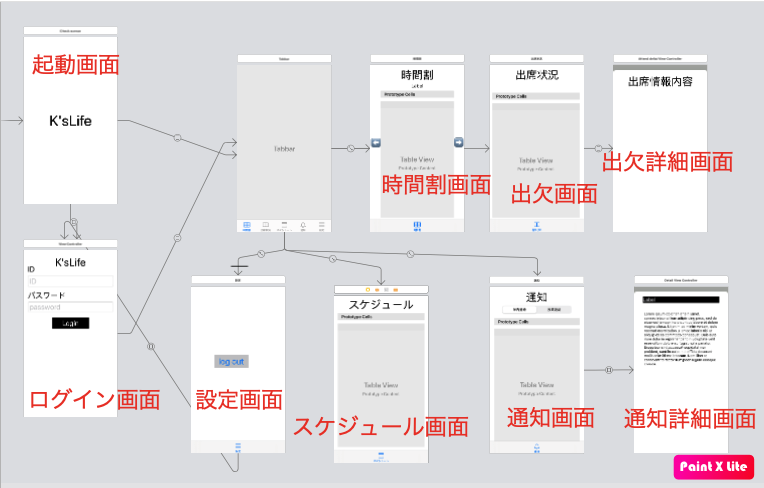
\includegraphics[clip,width = 10cm]{seni.png} %読み込む画像
  }
  \caption{画面遷移}\label{seni}
\end{figure}

\section{画面一覧}\label{rihabiri_jisso}
本節では、設計した画面について説明する。
\subsection{起動画面}
スマト君の起動画面である。起動画面を図\ref{kido}に示す。

\begin{figure}[htbp]
  \centering %中央寄せ
  \fbox{
    
\includegraphics[clip,width = 5cm]{1.jpg} %読み込む画像
  }
  \caption{起動画面}\label{kido}
\end{figure}

\subsection{ログイン画面}
スマト君へログインする画面である。ログイン画面を図\ref{login}に示す。

この画面は1にログイン用IDと2にパスワードを入力し、3のログインボタンを押すことで、ログイン成功すると時間割画面に遷移する。


\begin{figure}[htbp]
  \centering %中央寄せ
  \fbox{
    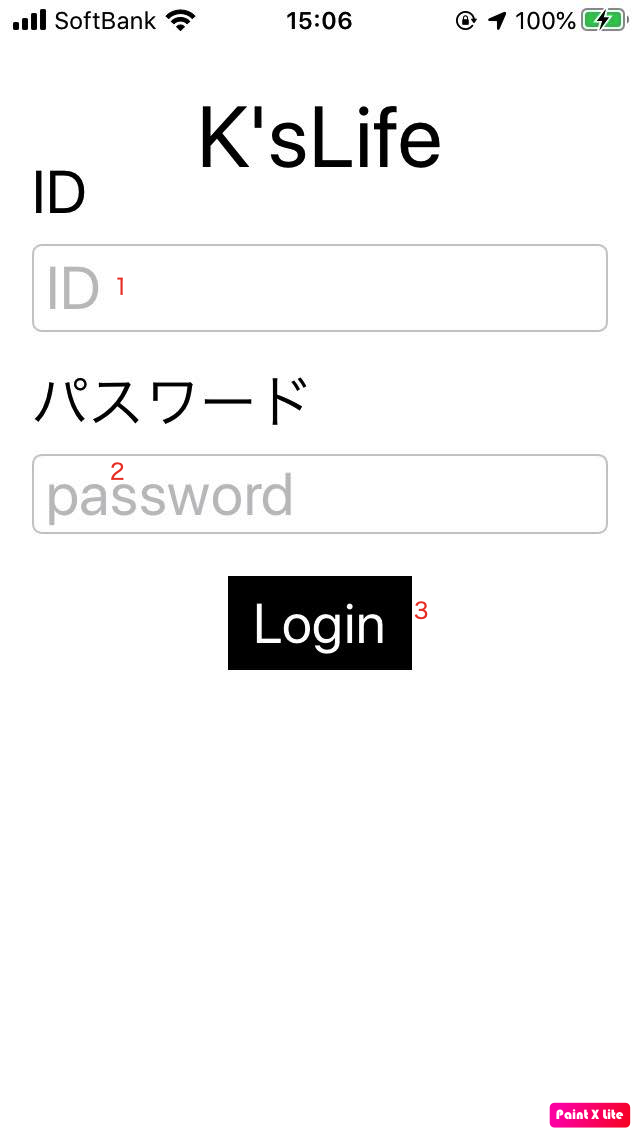
\includegraphics[clip,width = 5cm]{2.jpg} %読み込む画像
  }
  \caption{ログイン画面}\label{login}
\end{figure}

\subsection{時間割画面}
時間割が表示される画面である。時間割画面を図\ref{time}に示す。

 この画面はメニューバーがある。メニューバーの1を押すと時間割画面に遷移し、2を押すと出欠画面に遷移し、3を押すとスケジュール画面に遷移し、4を通知画面に遷移し、5を押すと設定画面に遷移する。
 6は曜日である。
 7は1日の時間割のテープルである。
8を押すと前日の時間割画面に遷移し、6、7の表示内容が変わる。
9を押すと翌日の時間割画面に遷移すし、6、7の表示内容が変わる。


\begin{figure}[htbp]
  \centering %中央寄せ
  \fbox{
    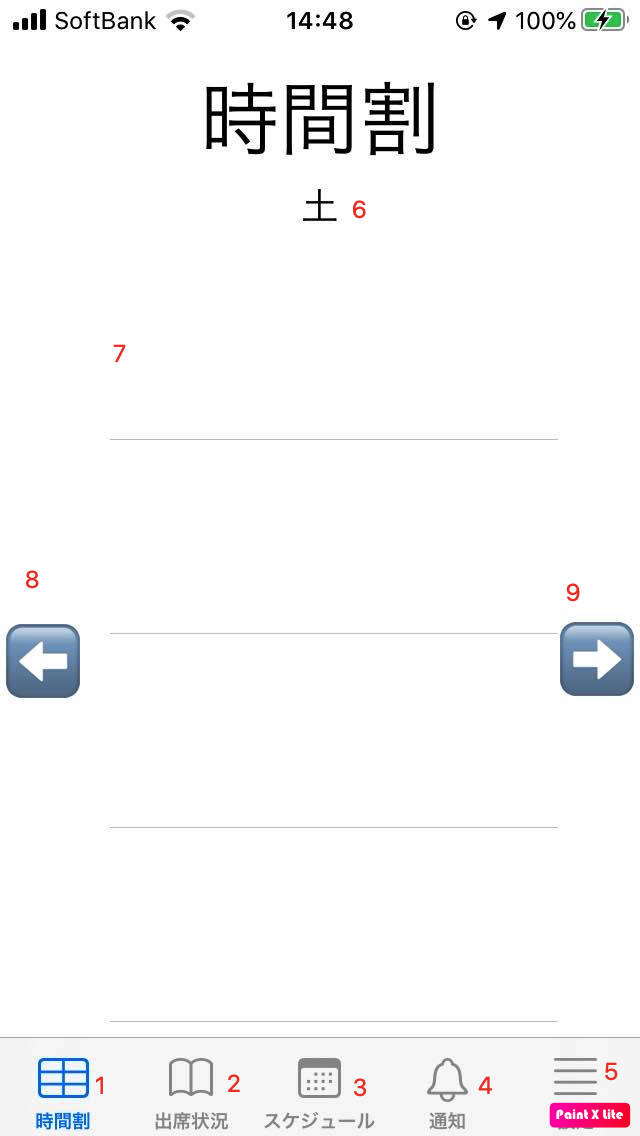
\includegraphics[clip,width = 5cm]{3.jpg} %読み込む画像
  }
  \caption{時間割画面}\label{time}
\end{figure}

\subsection{スケジュール画面}
スケジュールが表示される画面である。スケジュール画面を図\ref{suke}に示す。

この画面のメニューバーは5.3.3で述べたメニューバーと同じである。
6は1週間のスケジュールのテーブルである。

\begin{figure}[htbp]
  \centering %中央寄せ
  \fbox{
    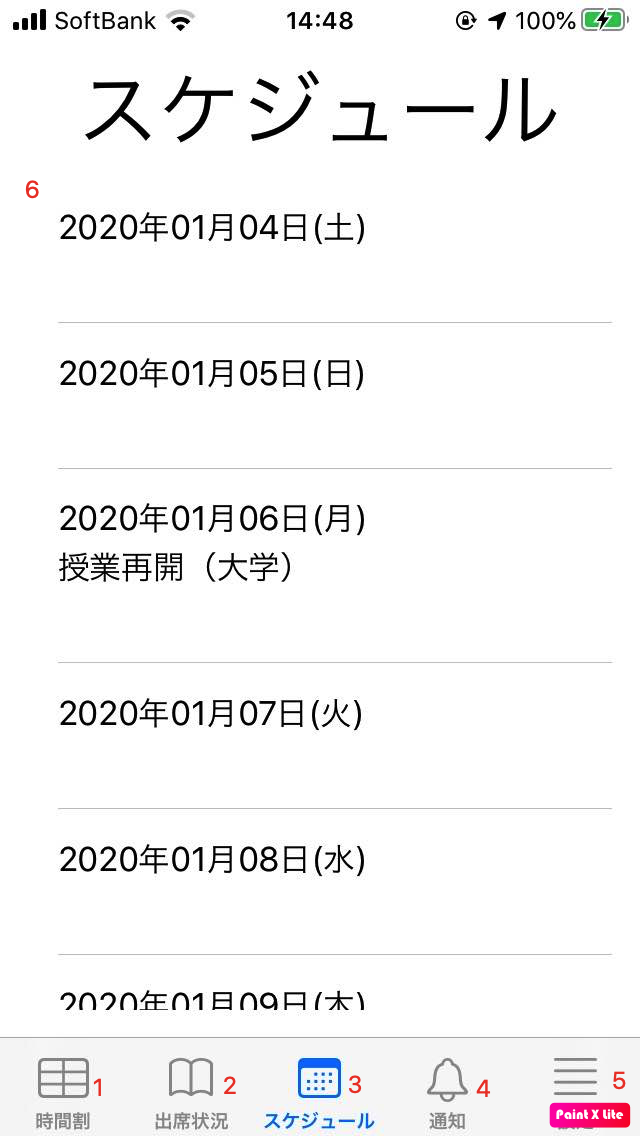
\includegraphics[clip,width = 5cm]{4.jpg} %読み込む画像
  }
  \caption{スケジュール画面}\label{suke}
\end{figure}

\subsection{出欠画面}
出欠情報が表示される画面である。出欠画面を図\ref{shuke}に示す。

この画面のメニューバーは5.3.3で述べたメニューバーと同じである。
6は履修中科目の一覧のテーブルであり、科目名を押すとその科目の出欠詳細画面に遷移する。

\begin{figure}[htbp]
  \centering %中央寄せ
  \fbox{
    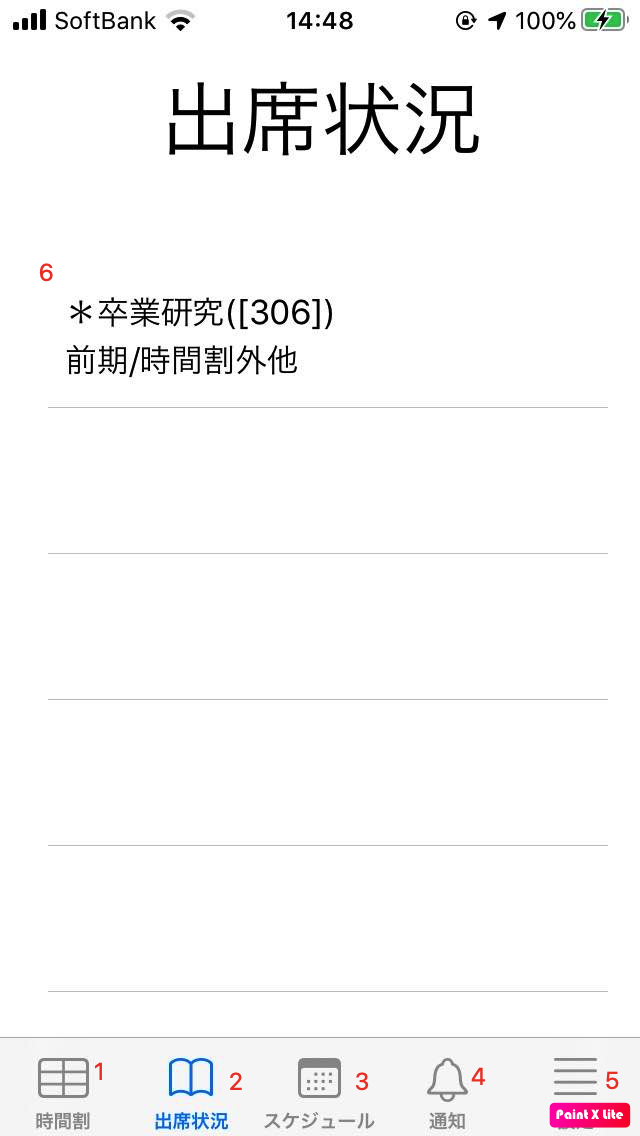
\includegraphics[clip,width = 5cm]{5.jpg} %読み込む画像
  }
  \caption{出欠画面}\label{shuke}
\end{figure}

\subsection{通知画面}
通知が表示される画面である。通知画面を図\ref{tuchi}に示す。

この画面のメニューバーは5.3.3で述べたメニューバーと同じである。
6の選択ボタンを押すと学内連絡に遷移し、7の選択ボタンを押すと授業連絡に遷移する。8は連絡のタイトル一覧のテープルであり、タイトルを押すと、この連絡の詳細画面に遷移する。


\begin{figure}[htbp]
  \centering %中央寄せ
  \fbox{
    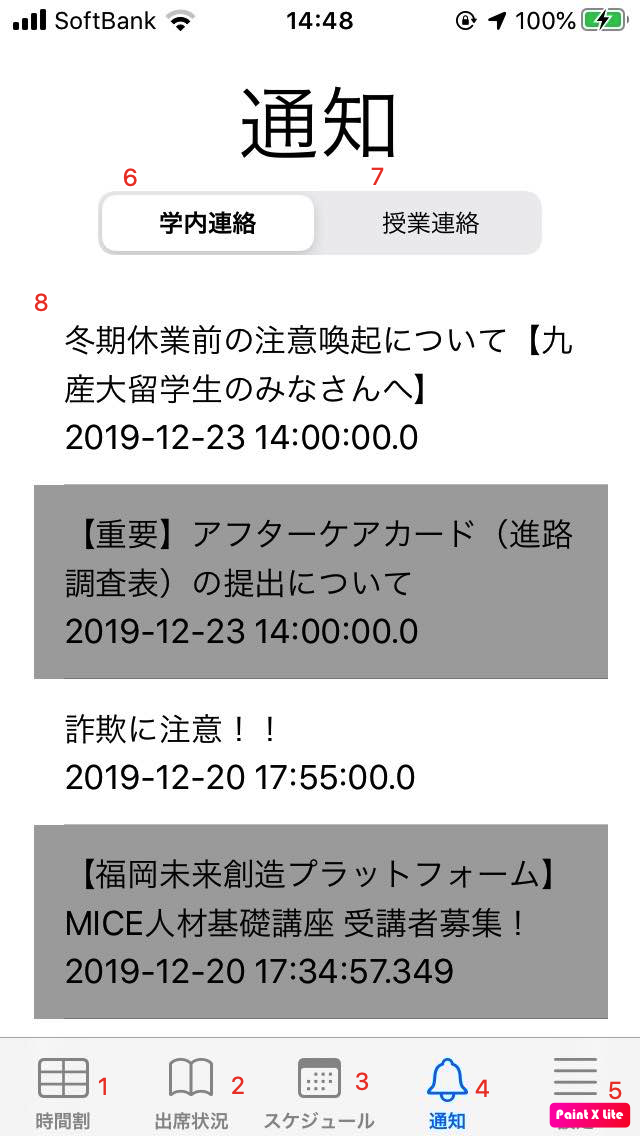
\includegraphics[clip,width = 5cm]{6.jpg} %読み込む画像
  }
  \caption{通知画面}\label{tuchi}
\end{figure}

\subsection{出欠詳細画面}
出欠詳細が表示される画面である。出欠詳細画面を図\ref{shuke_del}に示す。

この画面の1は出欠詳細情報である。上から下にスワイプすると出欠画面に遷移する。


\begin{figure}[htbp]
  \centering %中央寄せ
  \fbox{
    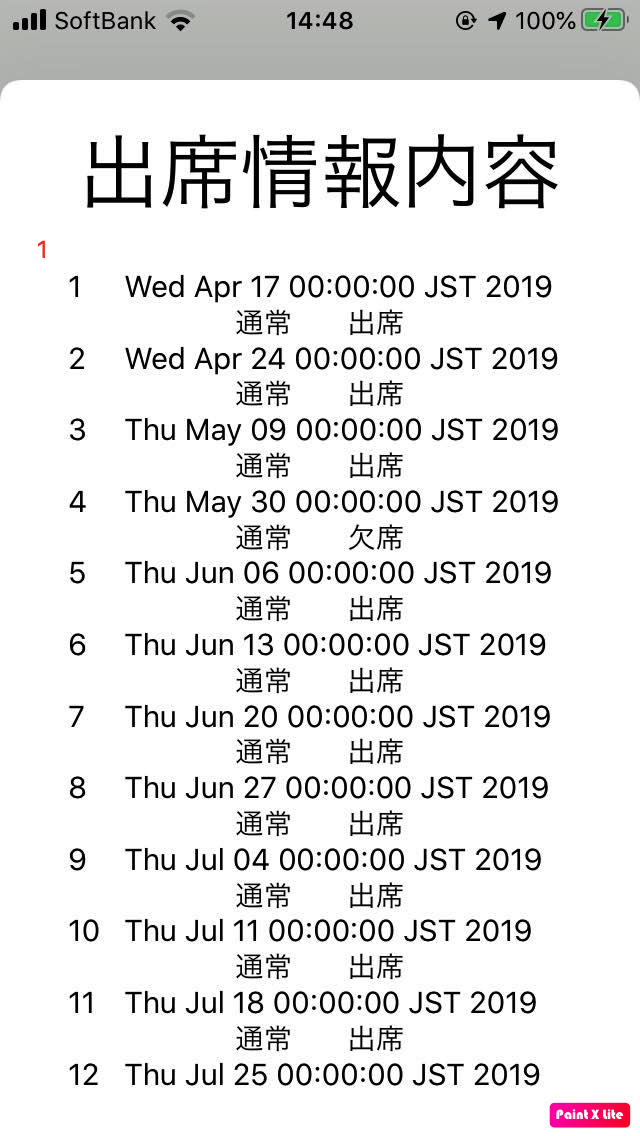
\includegraphics[clip,width = 5cm]{7.jpg} %読み込む画像
  }
  \caption{出欠詳細画面}\label{shuke_del}
\end{figure}

\subsection{連絡詳細画面}
通知詳細が表示される画面である。通知詳細画面を図\ref{tuchi_del}に示す。

この画面の1は通知のタイトルであり。2は詳細通知である。上から下にスワイプすると連絡画面に遷移する。


\begin{figure}[htbp]
  \centering %中央寄せ
  \fbox{
    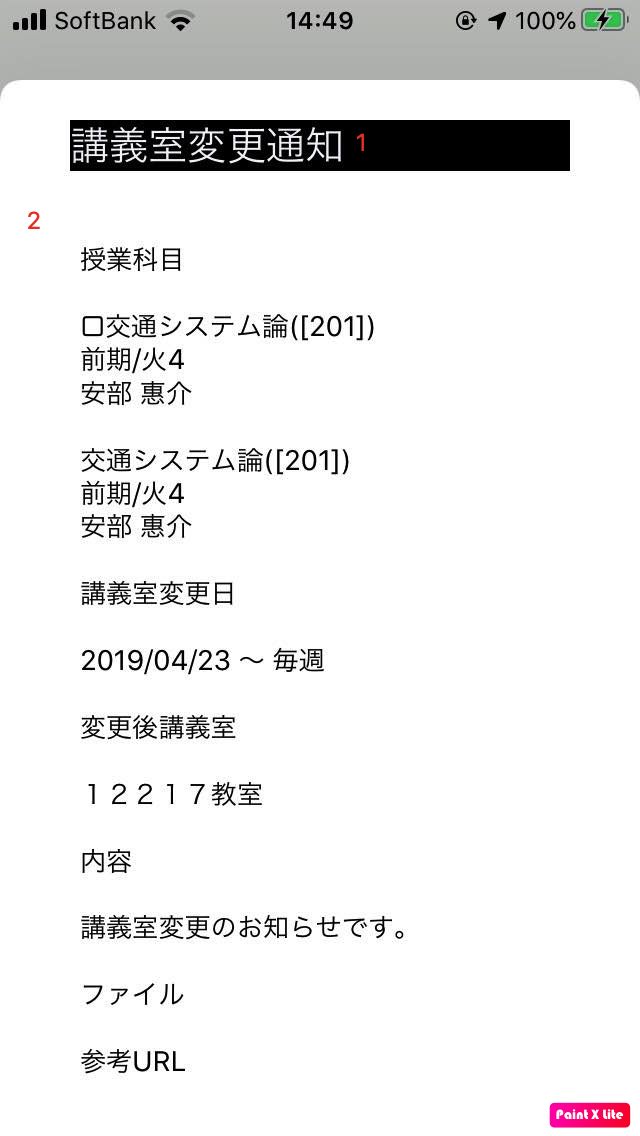
\includegraphics[clip,width = 5cm]{8.jpg} %読み込む画像
  }
  \caption{連絡詳細画面}\label{tuchi_del}
\end{figure}

\subsection{設定画面}
スマト君の設定画面である。設定画面を図\ref{set}に示す。

この画面の6のログアウトボタンを押すと、ログアウトしてログイン画面に遷移する。


\begin{figure}[htbp]
  \centering %中央寄せ
  \fbox{
    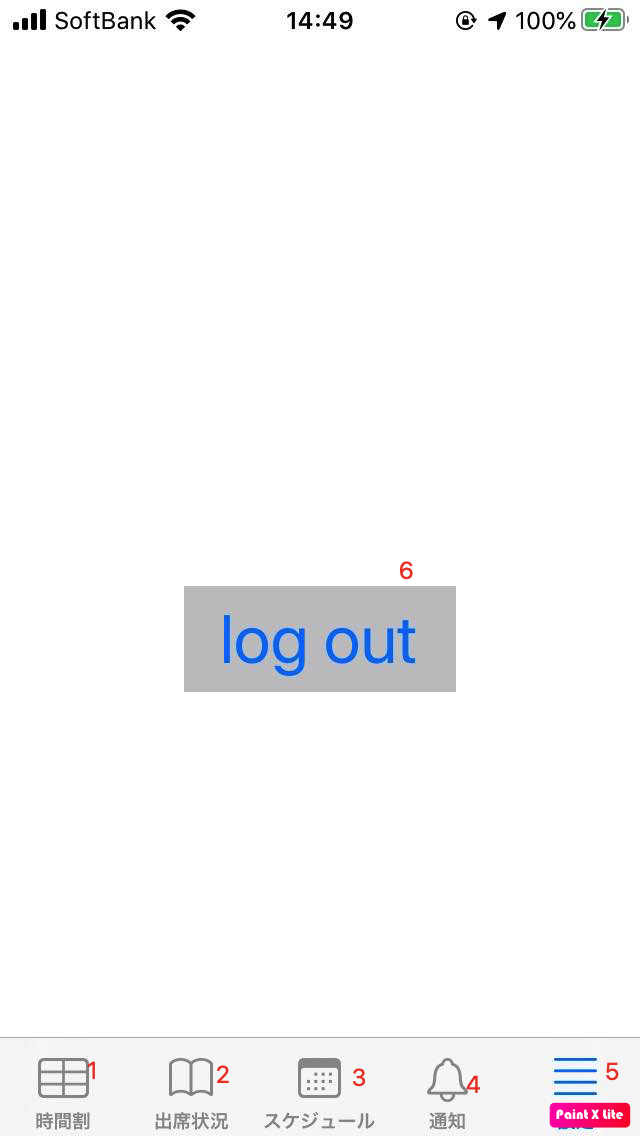
\includegraphics[clip,width = 5cm]{9.jpg} %読み込む画像
  }
  \caption{設定画面}\label{set}
\end{figure}

\section{スマト君アプリケーションの開発環境}\label{rihabiri_jisso}
本節はスマト君アプリケーションの開発環境について述べる。

\subsection{Xcode}
Xcode\cite{xcode}は、Apple社が開発しているアプリ開発ツールである。

MacやiPhone、iPadなどのアプリケーション開発に必要なものがすべて詰め込まれている。


\subsection{Swift}
Swift\cite{swift}とは、ネイティブアプリを開発するためのプログラミング言語である。
対象としているOSは、MacOSとiOSである。
iPhoneやiPadなどの端末で使えるアプリ、もしくはMacパソコン向けのアプリを開発ができる。

\section{スマト君アプリケーション実装}\label{rihabiri_jisso}
名前、学籍番号、時間割を取得API を呼ぶ。その API の返り値を使って、空値場合はログイン失敗、ログイン画面をそのままに表示、空でない値場合は時間割画面を表示してId、passwordは簡単なデータベースのUserDefaultでを保存する、出欠、スケジュール、連絡通知を取得APIを呼ぶ。
出欠情報画面に科目の一覧のテーブルがある。科目を押しと出欠詳細を取得APIを呼ぶ、出欠詳細画面に表示する。
通知画面に情報の一覧のテーブルがある。タイトルを押しと学内連絡か授業連絡詳細を取得APIを呼ぶ、通知詳細画面に表示する。
通知画面にはもともと15個通知しかないで、もと見るを押しと学内連絡か授業連絡を取得APIを呼ぶ、5個通知追加して表示する。
設定画面にあるログアウトボタンを押しと、UserDefaultで保存した情報を削除して、ログイン画面に表示する。
ログアウトしないでアプリを再起動すると時間割画面を表示して、出欠、スケジュール、連絡通知を取得APIを呼ぶ。前回を取った最新通知と今回取った最新通知と比較して、等しくないなら、notificationを出す。
Swiftにはlocal notificationとpush notificationがある。
15分単位で出欠、スケジュール、連絡通知を取得APIを定期呼んでlocal notificationを出すと思うが、Swiftはアプリを出ると最大30秒だけバックグラウンドで実行する。このため通知機能はアプリ起動するときだけできて、うまく出来ない。
push notificationの場合はserverで定期実行、firebaseAPNをrequest方法を調べた。しかし、serverでIDとpasswordを使用するので、セキュリティーに危険なので、使用しなっかた。

%-----------------------------------------------------------------------------------------------------------------

\chapter{評価}\label{hyoka}
本章では、スマト君の評価について述べる。

\section{評価方法}\label{rihabiri_jisso}
下川研のメンバーに利用してもらい、アンケート結果をまとめた。
アンケートの内容は以下のとおりである

\begin{enumerate}
  \item スマト君について、簡単さ、便利さ、動作のスピードを5点満点で評価
  \item スマト君を使用することでブラウザで K'sLifeを使うよりも操作は簡単になるか、見易くなるかを評価
  \item スマト君を続けて使用したいかを評価
\end{enumerate}

\section{評価結果}\label{rihabiri_jisso}
8人にスマト君を使ってもらった。

スマト君を使用することで操作は K'sLifeよりも簡単になったと評価した人は  62.5 \%、あまり変わらないと評価した人は37.5\%、難しいと評価した人は0\%。
この結果を図\ref{sosa}に示す。


\begin{figure}[htbp]
  \centering %中央寄せ
  \fbox{
    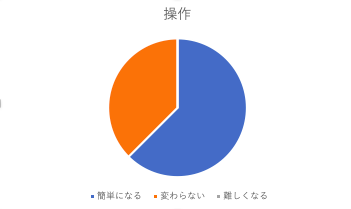
\includegraphics[clip,width =  10cm]{sosa.png} %読み込む画像
  }
  \caption{スマト君の操作の評価}\label{sosa}
\end{figure}

 スマト君のデザインはスマートフォンで K'sLifeを見るよりも見やすいと評価した人は 62.5 \%、あまり変わらないと評価した人は37.5\%、見にくいと評価した人は0\%。
  この結果を図\ref{dezai}に示す。


 \begin{figure}[htbp]
   \centering %中央寄せ
   \fbox{
     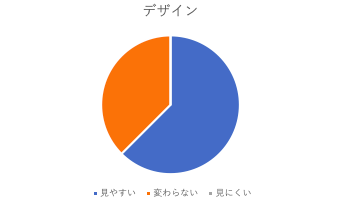
\includegraphics[clip,width =  10cm]{dezai.png} %読み込む画像
   }
   \caption{スマト君のデザインの評価}\label{dezai}
 \end{figure}

続けて使用したい人は 12.5 \%、どちらでもいいと考える人は87.5\%、使用したくない人は0\%。
この結果を図\ref{siyou}に示す。


\begin{figure}[htbp]
  \centering %中央寄せ
  \fbox{
    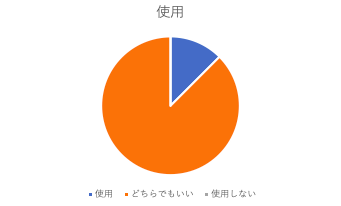
\includegraphics[clip,width =  10cm]{siyou.png} %読み込む画像
  }
  \caption{スマト君を続けて使用したいの結果}\label{siyou}
\end{figure}

スマト君について、簡単さ、便利さ、動作のスピードを5点満点で評価は平均点をまとめて、表\ref{keka}と図\ref{kurafu}に示す。


\begin{table}[htbp]
\caption{スマト君の評価}
\centering
\begin{tabular}{|l|l|l|l|}
\hline
    & 簡単 & 便利 & スピード \\ \hline
平均点 &  \multicolumn{1}{r|}  {3.6}   & \multicolumn{1}{r|}{3.9}	   & \multicolumn{1}{r|}{3.9}    \\ \hline
\end{tabular}
\label{keka}
\end{table}

\begin{figure}[htbp]
  \centering %中央寄せ
  \fbox{
    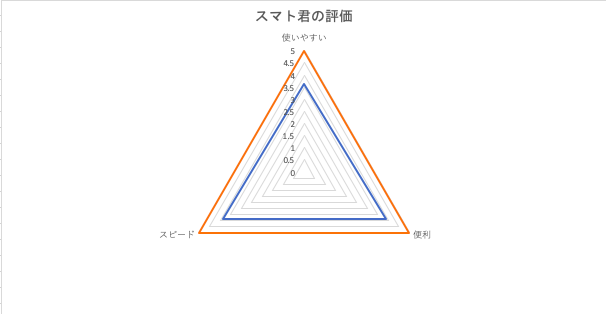
\includegraphics[clip,width =  10cm]{10.png} %読み込む画像
  }
  \caption{スマト君全体の評価}\label{kurafu}
\end{figure}

\section{考察}\label{rihabiri_jisso}
表6.1 より、高い評価を得ることができた。

スマト君の操作しやすさと、デザインは、良い評価が半分以上である。2.1で述べた問題点は解決できたと考える。
しかし、続けて使用したいと考えている人は少ない。
スマト君を使ってもらった人たちはほとんど4年生である。卒業するのため、K'sLifeをあまり使わなくなる。この理由でどちらでもいいと回答した人が多い。



%-----------------------------------------------------------------------------------------------------------------

\chapter{結論}\label{keturon}
本章では、本研究のまとめと今後の課題について述べる。

\section{まとめ}\label{matome}
九州産業大学では、学生教育支援・事務情報システム K'sLifeを運用している。
K'sLife をスマートフォンで使用する際、問題点がある。
そこで、本研究では、スマートフォン用K'sLifeアプリを開発した。
このシステムを「スマト君」と名付けた。

スマト君は、K'sLife の API を提供するための 「スマト君 API Server」と、
スマートフォン用アプリケーションである「スマト君アプリケーション」と、
従来の K'sLife から構成される。

スマト君を実際に利用してもらい、アンケートで評価した。
評価結果から、高評価を得た。
しかし、まだ改善が必要である。
\section{今後の課題}\label{kadai}
スマト君に機能はまだ少ない、デザインはシンプルである。このため、スマト君の機能を追加し、デザインを修正することは必要と考える。
そして、Androidを使用している人もいる。誰でも使えるようにするためAndroid用アプリケーションの開発が必要である。

\chapter*{謝辞}
本研究を進めるにあたり、ご指導をいただいた九州産業大学理工学部情報科学科の下川俊彦教授、神屋郁子講師に感謝いたします。

そして、日常の議論を通じて多くの知識や示唆を頂いた下川研究室の皆様に感謝致します。

\begin{thebibliography}{99}%参考文献の数が1桁なら9,3桁なら999にする
\bibitem{kslife}学生教育支援・事務情報システム K'sLife \url{https://ksuweb.kyusan-u.ac.jp/}


  \bibitem {ubuntu} Ubuntu
  \url{https://www.ubuntulinux.jp/}

  \bibitem {nodejs} Node.js
  \url{https://nodejs.org/}

  \bibitem {puppeteer} Puppeteer
  \url{https://github.com/puppeteer/puppeteer}

  \bibitem {express} Express
  \url{https://expressjs.com/ja/}

  \bibitem {xcode} Xcode
  \url{https://developer.apple.com/jp/xcode/}

  \bibitem {swift} Swift
  \url{https://www.apple.com/jp/swift/}


\end{thebibliography}
\appendix
\chapter{スマト君の評価アンケート}\label{hyouka}
\begin{verbatim}
スマト君の評価アンケート
 このアンケートは、スマートフォン用K'sLifeアプリ「スマト君」の評価を貰うためのものです。
本アンケートに回答お願いします。
*必須
スマト君は使いやすいですか?(5点満点で採点してください) *
1 つだけマークしてください。
 1
 2
 3
 4
 5
スマト君は便利ですか?(5点満点で採点してください) *
1 つだけマークしてください。
 1
 2
 3
 4
 5
スマト君の操作のスピードはどうですか?(5点満点で採点してください) *
1 つだけマークしてください。
 1
 2
 3
 4
 5
スマト君を使用することでブラウザで K'sLifeを使うよりも操作は簡単になりましたか? *
1 つだけマークしてください。
 簡単になった
 あまり変わらない
 難しくなった
スマト君のデザインはスマートフォンで K'sLifeを見るよりも見やすいですか? *
1 つだけマークしてください。
 見やすい
 あまり変わらない
 見にくい
スマト君を続けて使用したいと思いますか? *
1 つだけマークしてください。
 使用します
 どちらでもいい
 使用したくない
その他、本システムについて意見があれば、記入してくだい。

\end{verbatim}
\end{document}
